\documentclass[a4paper, 11pt]{article}
\usepackage[polish]{babel}
\usepackage[T1]{fontenc}
\usepackage{hyperref}
\usepackage{array}
\usepackage{amssymb}
\usepackage[margin=1in]{geometry}
\hypersetup{
    colorlinks,
    citecolor=black,
    filecolor=black,
    linkcolor=black,
    urlcolor=black
}
\usepackage{graphicx}

\usepackage{tikz}
\usetikzlibrary{fit,arrows,matrix,positioning, calc, shapes.gates.logic.IEC, shapes.gates.logic.US}
\tikzstyle{branch}=[fill,shape=circle,minimum size=3pt,inner sep=0pt]


\title{%
	\vspace{-1.5cm}
       \large Sprawozdanie Laboratorium Mikroelektronika \\
       \huge  Podstawowe symulacje wybranych układów CMOS}

\author{Stanisław Fiedler 160250 L1}
\date{LAB 5, 19 listopada 2024}

\begin{document}

\maketitle
\tableofcontents

\section{Bramka NAND}\label{sec:nand} % (fold)
Dla symulacji układu z rysunku 1 wyznaczyć parametry rise time, fall time, edge rate,
high-to-low propagation delay, low-to-high propagation delay, propagation delay, contamination delay.
\subsection{Wyniki symulacji}\label{sub:wyniki_symulacji} % (fold)
\begin{center}
	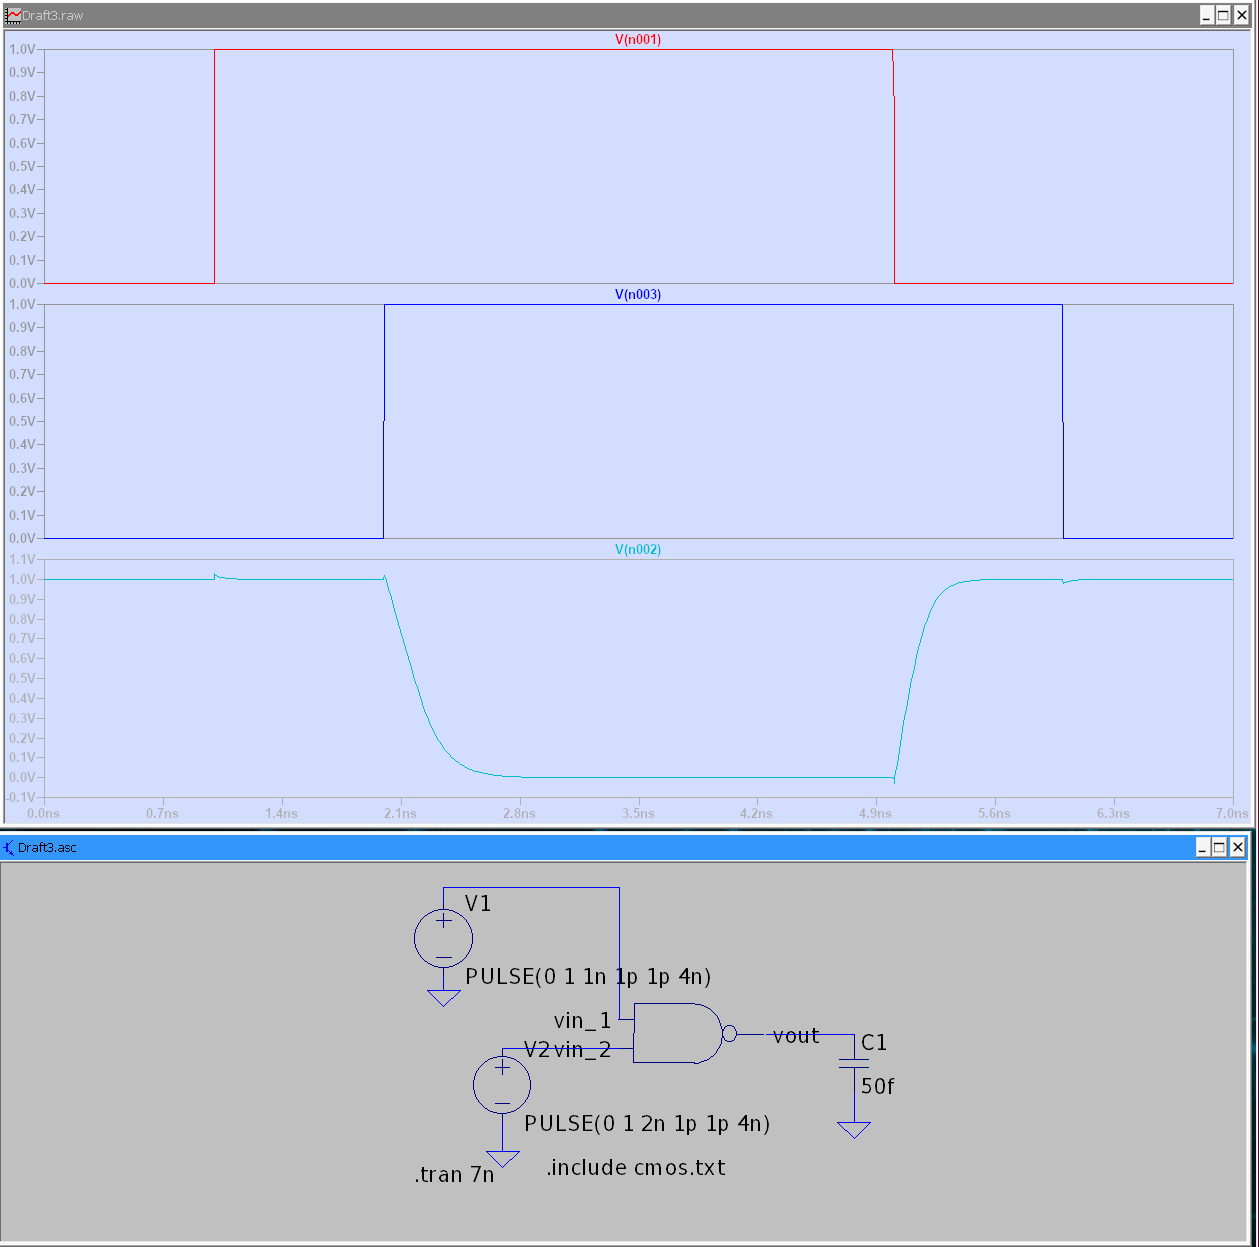
\includegraphics[scale=0.27]{images/nand.png}
\end{center}
% subsection Wyniki symulacji (end)
\subsection{Tablica prawdy}\label{sub:tablica_prawdy} % (fold)
\begin{center}
	\begin{tabular}{c|c|c}
		A & B & A nand B \\
		\hline
		0 & 0 & 1        \\
		0 & 1 & 1        \\
		1 & 1 & 0        \\
		1 & 0 & 1        \\
	\end{tabular}
\end{center}
% subsection Tablica prawdy (end)
\subsection{Wyznaczone parametry}\label{sub:wyznaczone_parametry} % (fold)
\begin{description}
	\item[Rise time:] $175ps$ \hfill
	      \begin{center}
		      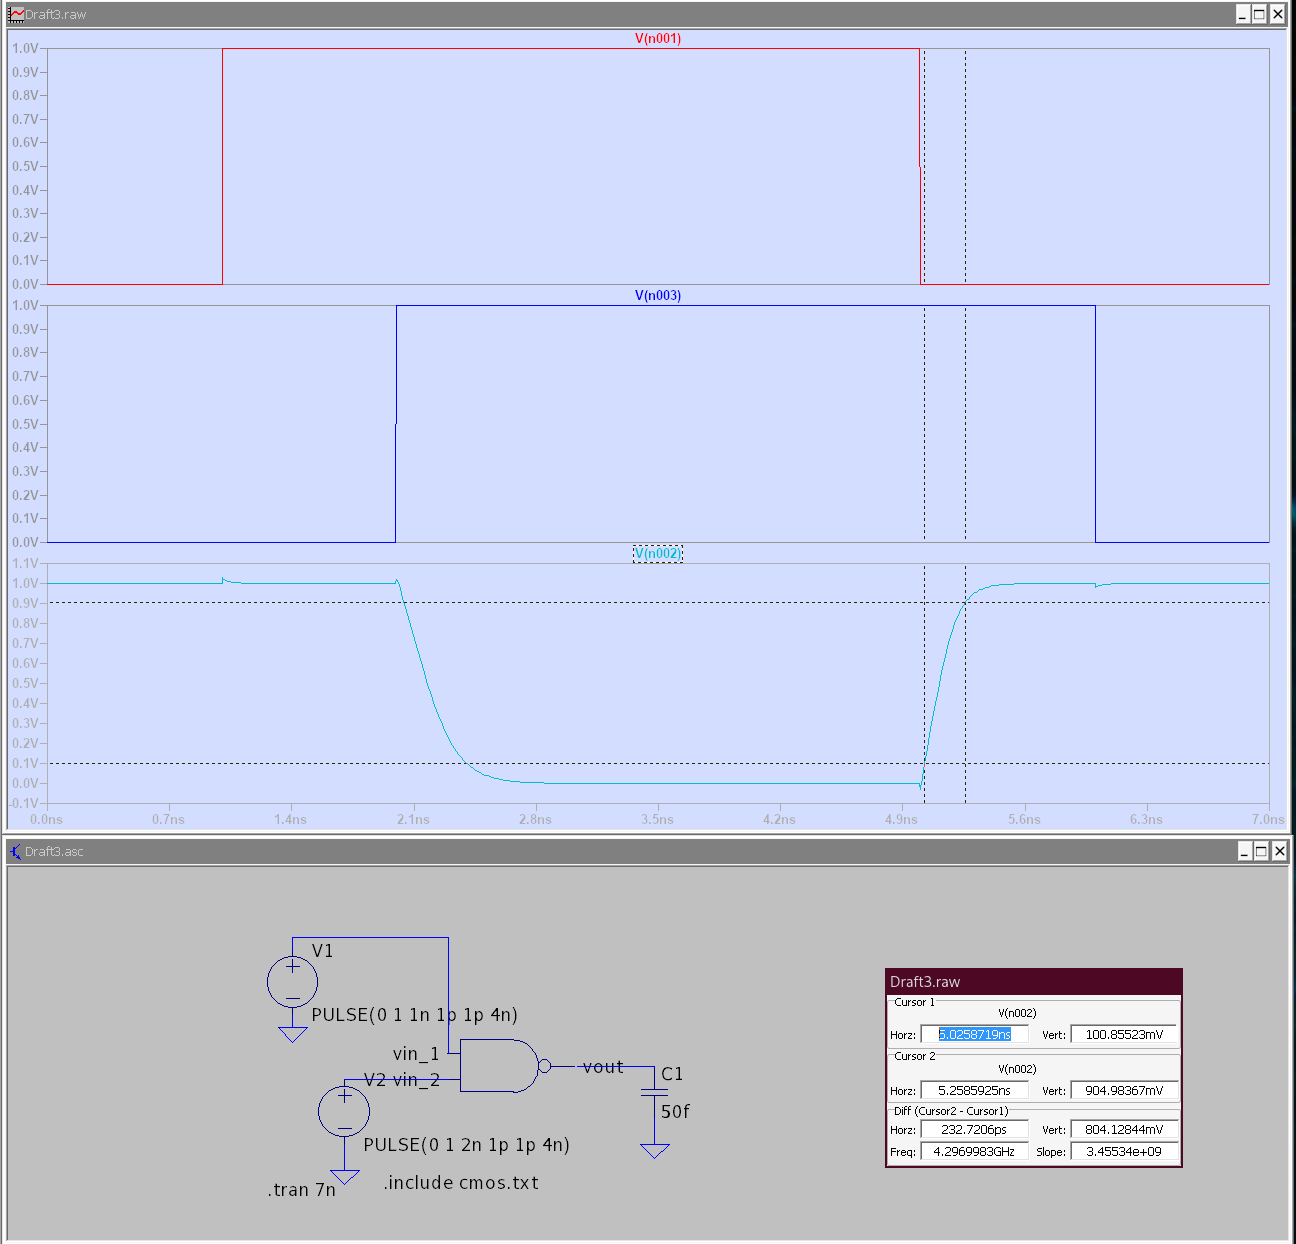
\includegraphics[scale=0.29]{images/rise_time.png}
	      \end{center}
	\item[Fall time:] $1,35 \, ns$ \hfill
	      \begin{center}
		      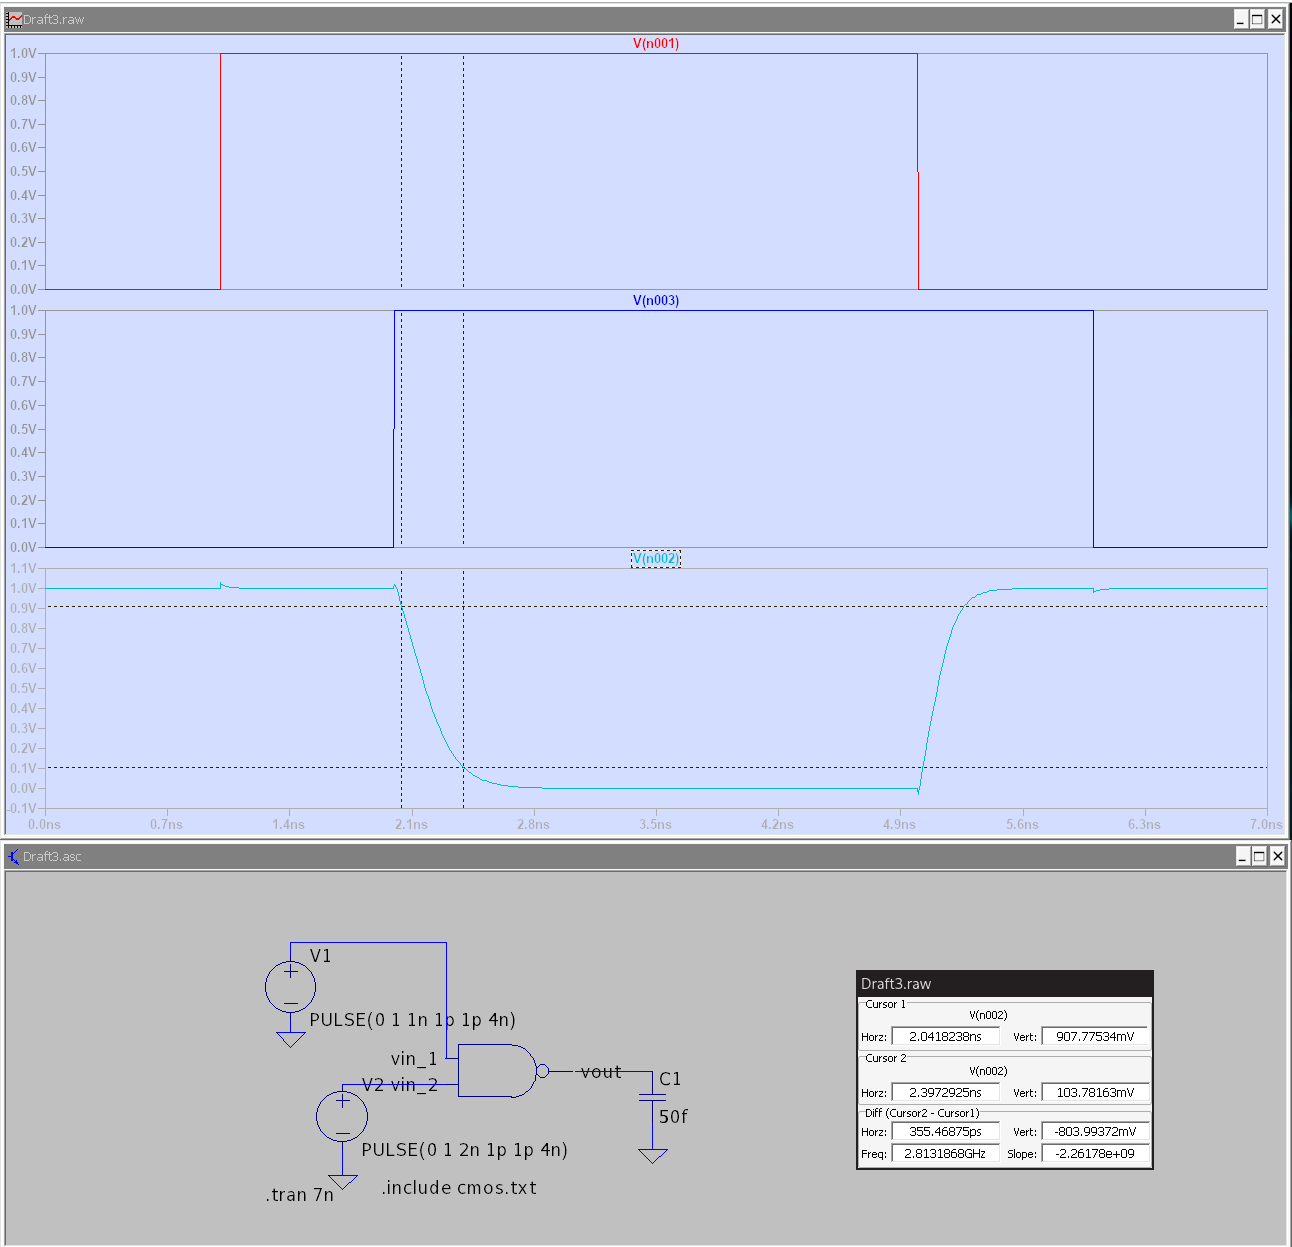
\includegraphics[scale=0.29]{images/fall_time.png}
	      \end{center}
	\item[Edge rate:] $\frac{175ps + 1350ps}{2} = 763ps$
	\item[High-to-low propagation delay:] $547ps$ \hfill
	      \begin{center}
		      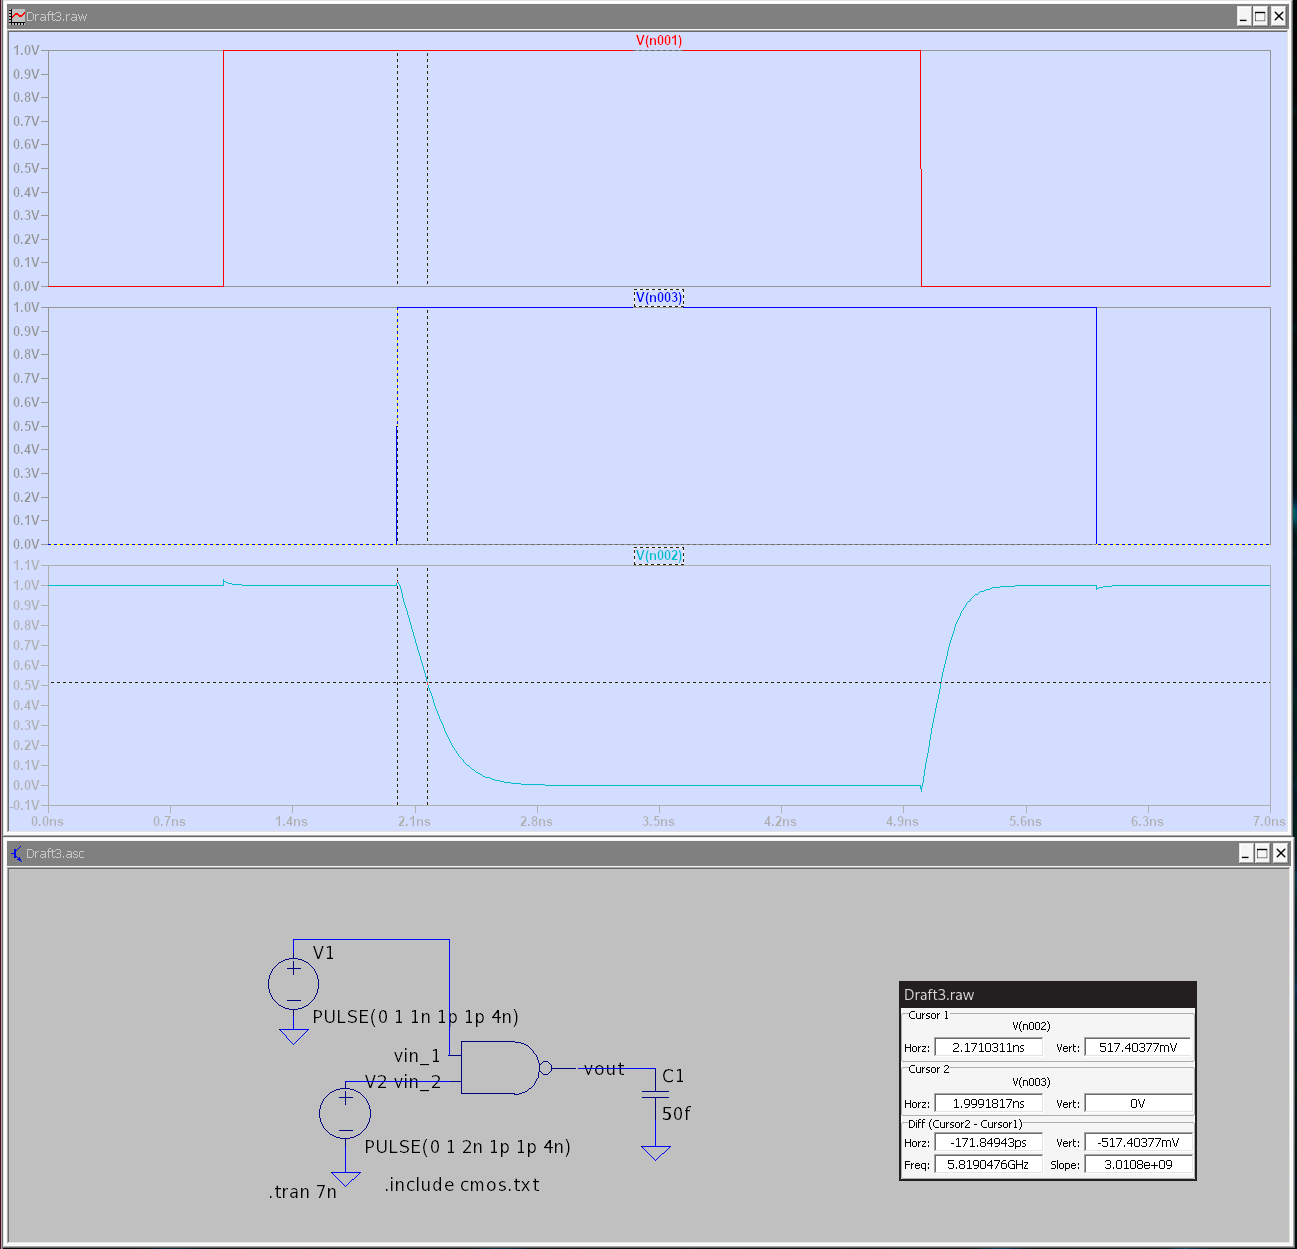
\includegraphics[scale=0.3]{images/high_to_low.png}
	      \end{center}
	\item[Low-to-high propagation delay:] $143ps$ \hfill
	      \begin{center}
		      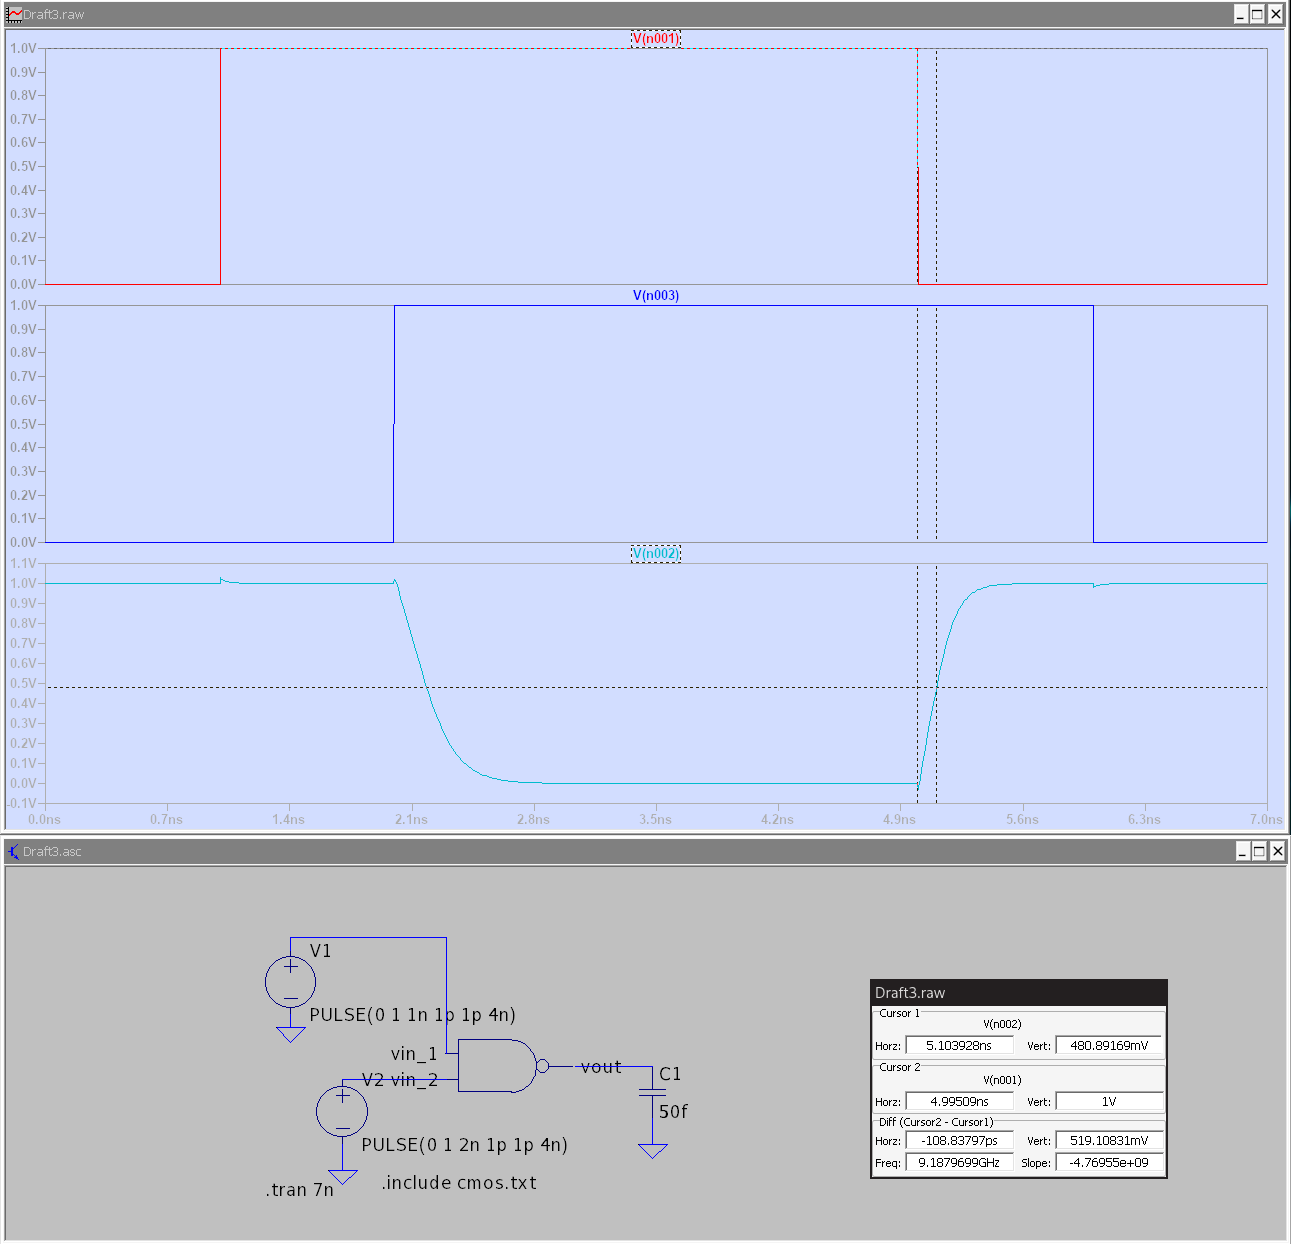
\includegraphics[scale=0.3]{images/low_to_high.png}
	      \end{center}
	\item[Propagation delay:] $\frac{547ps + 143ps}{2} = 345ps $
	\item[Contamination delay:] $ min\{143ps, 547ps\} = 143ps $
\end{description}
% subsection Wyznaczone parametry (end)
% section NAND (end)

\section{Bramka AND}\label{sec:and} % (fold)
Zaprojektować na tranzystorach nmos4 i pmos4 bramkę AND (bez projektowania symbolu). Zaprojektować
układ do testowania bramki oraz dokonać jej symulacji, w której sygnały pobudzenia będą reprezentowały
wszystkie kombinacje z tabeli prawdy.
\subsection{Wyniki symulacji}\label{sub:wyniki_symulacji} % (fold)
\begin{center}
	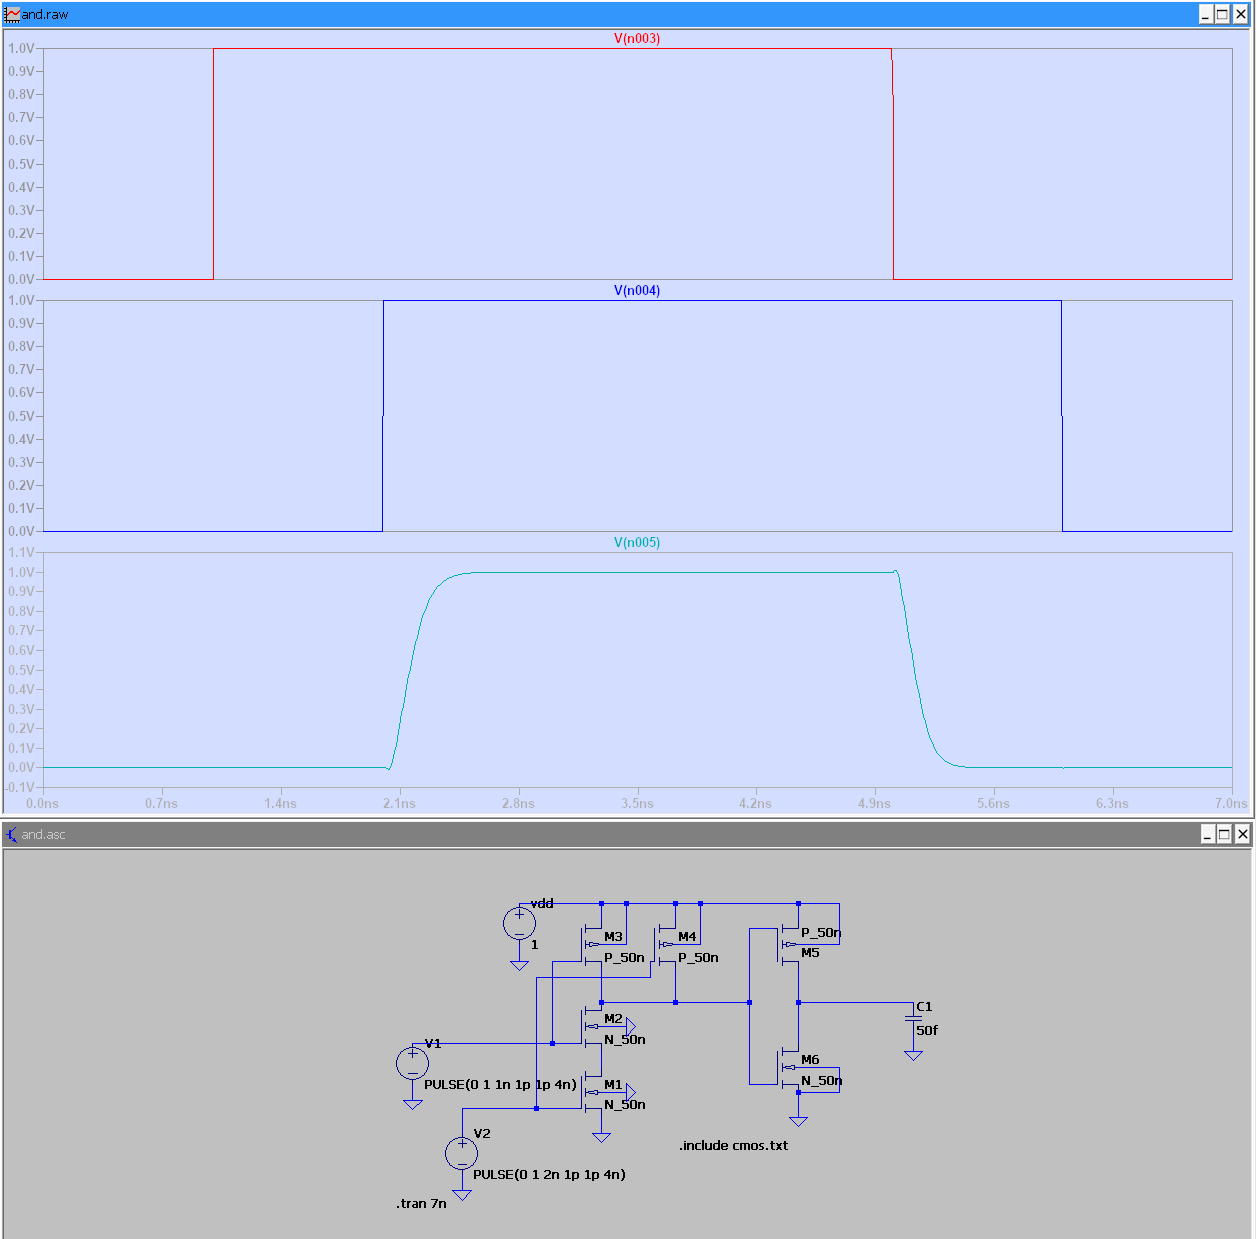
\includegraphics[scale=0.35]{images/and.png}
\end{center}
% subsection Wyniki symulacji (end)
\subsection{Tablica prawdy}\label{sub:tablica_prawdy} % (fold)
\begin{center}
	\begin{tabular}{c|c|c}
		A & B & A and B \\
		\hline
		0 & 0 & 0       \\
		0 & 1 & 0       \\
		1 & 1 & 1       \\
		1 & 0 & 0       \\
	\end{tabular}
\end{center}
% subsection Tablica prawdy (end)
% section AND (end)

\pagebreak
\section{Bramka NOR}\label{sec:bramka_nor} % (fold)
Zaprojektować na tranzystorach nmos4 i pmos4 bramkę NOR (bez projektowania symbolu). Zaprojektować
układ do testowania bramki oraz dokonać jej symulacji, w której sygnały pobudzenia będą reprezentowały
wszystkie kombinacje z tabeli prawdy.
\subsection{Wyniki symulacji}\label{sub:wyniki_symulacji} % (fold)
\begin{center}
	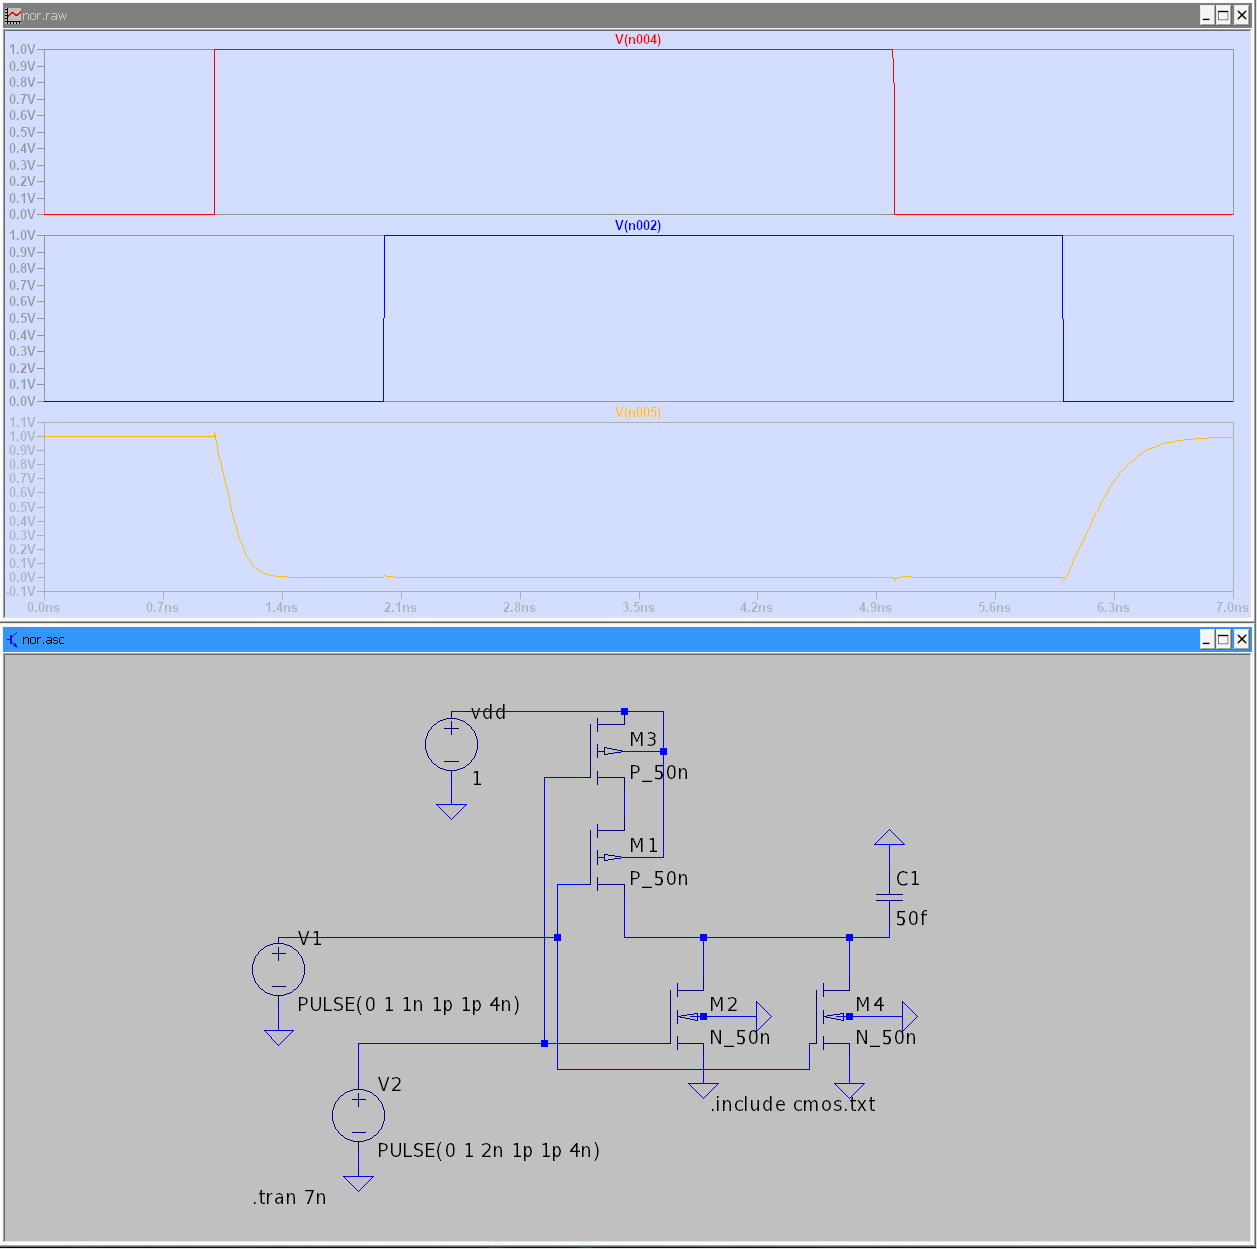
\includegraphics[scale=0.35]{images/nor.png}
\end{center}
% subsection Wyniki symulacji (end)
\subsection{Tablica prawdy}\label{sub:tablica_prawdy} % (fold)
\begin{center}
	\begin{tabular}{c|c|c}
		A & B & A nor B \\
		\hline
		0 & 0 & 1       \\
		0 & 1 & 0       \\
		1 & 1 & 0       \\
		1 & 0 & 0       \\
	\end{tabular}
\end{center}
% subsection Tablica prawdy (end)
% section Bramka NOR (end)

\end{document}

